\documentclass[]{IEEEtran}
% some very useful LaTeX packages include:
%\usepackage{cite}      
\usepackage{graphicx}   
\usepackage{subfigure} 
\usepackage{url}       
\usepackage{amsmath}    
\usepackage{caption2}
% Your document starts here!
\begin{document}

% Define document title and author
	\title{Weekly Report}
	\author{Adviser: Prof. Yang Wen \\Student: Cheng Wensheng\\ Period: 2018.6.24-7.1
	}
	\markboth{Visual Information Processing Group}{}
	\maketitle

% Write abstract here
\begin{abstract}
	This week I mainly put my effort on processing SAR data of Shanghai.
\end{abstract}

% Each section begins with a \section{title} command
\section{Data process}
	% \PARstart{}{} creates a tall first letter for this first paragraph
	\PARstart{F}{or} this SAR contest, since the contest committee hasn't launched the training data, we need to label some data manually. We already have the SAR data of Shanghai City, considering future project of change detection, so we plan to label this.

	Basically, we have the SAR data of Shanghai City in December, 2013. With Google Earth software, we can get corresponding optical satellite image at the same time. With the help of optical image, we can label SAR data accurately.
	
	However, to map the SAR data region to corresponding optical image on Google Earth, we need to geocode the SAR image first. The point of view of SAR image is different with that of optical image, so we need to calibrate it to optical image and change its coordinates to the latter. After this, we can split the SAR and optical image with the same manner, then it's feasible to label smaller SAR images with pairwise optical reference images.

	Peng Rui has learned the method of calibration, but he said that he lacks some primitive SAR data of Shanghai City to do geocoding. And we think Prof. Yang could have these data, so we'll continue our labeling work after we get these data for geocoding.
	
	Fig.~\ref{fig:fw} is Shanghai City image in the software. 
	

% Main Part

\newpage
\begin{figure}[!hbt]
%		 Center the figure.
		\vspace{1.7cm}
%		\hspace{50cm}
		\begin{center}
			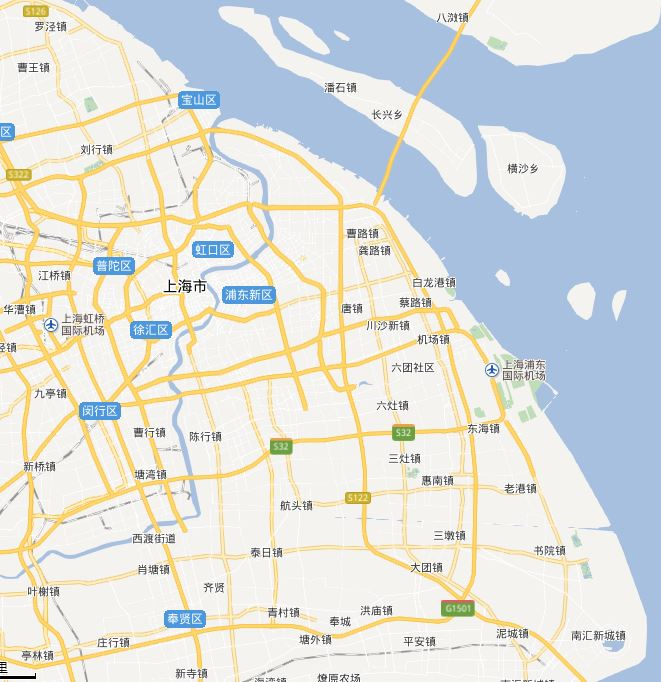
\includegraphics[width=\columnwidth]{op}
				%		 Create a subtitle for the figure.
			\caption{Shanghai City image in the software.}
			\label{fig:fw}
		    
		\end{center}
	\end{figure}

% Now we need a bibliography:
%\begin{thebibliography}{5}
%
%	%Each item starts with a \bibitem{reference} command and the details thereafter.
%	\bibitem{HOP96} % Transaction paper
%	J.~Hagenauer, E.~Offer, and L.~Papke. Iterative decoding of binary block
%	and convolutional codes. {\em IEEE Trans. Inform. Theory},
%	vol.~42, no.~2, pp.~429–-445, Mar. 1996.
%
%	\bibitem{MJH06} % Conference paper
%	T.~Mayer, H.~Jenkac, and J.~Hagenauer. Turbo base-station cooperation for intercell interference cancellation. {\em IEEE Int. Conf. Commun. (ICC)}, Istanbul, Turkey, pp.~356--361, June 2006.
%
%	\bibitem{Proakis} % Book
%	J.~G.~Proakis. {\em Digital Communications}. McGraw-Hill Book Co.,
%	New York, USA, 3rd edition, 1995.
%
%	\bibitem{talk} % Web document
%	F.~R.~Kschischang. Giving a talk: Guidelines for the Preparation and Presentation of Technical Seminars.
%	\url{http://www.comm.toronto.edu/frank/guide/guide.pdf}.
%
%	\bibitem{5}
%	IEEE Transactions \LaTeX and Microsoft Word Style Files.
%	\url{http://www.ieee.org/web/publications/authors/transjnl/index.html}
%
%\end{thebibliography}

% Your document ends here!
\end{document}